\documentclass[%
 reprint,
superscriptaddress,
groupedaddress,
%unsortedaddress,
%runinaddress,
%frontmatterverbose, 
%preprint,
%preprintnumbers,
%nofootinbib,
%nobibnotes,
%bibnotes,
 amsmath,amssymb,
 aps,
prl
%prb,
%rmp,
%prstab,
%prstper,
%floatfix,
]{revtex4-2}

\usepackage{graphicx}% Include figure files
\usepackage{dcolumn}% Align table columns on decimal point
\usepackage{bm}% bold math
\usepackage{braket}
\usepackage{color}
\graphicspath{{./figures/}}
\bibliographystyle{apsrev4-2}

\begin{document}

\title{Pseudogapped non-Fermi liquid phase arising from Kondo breakdown at the Mott transition}

%\title{What lies between a Fermi liquid and a Mott insulator in two dimensions? Insights from an impurity model}% Force line breaks with \\

\author{Abhirup Mukherjee}
\author{Siddhartha Lal}
\affiliation{%
 Department of Physical Sciences, Indian Institute of Science Education and Research Kolkata, Nadia - 741246, India
}%

\date{\today}
\begin{abstract}
We present an auxiliary model approach that illuminates the centrality of the pseudogap phenomenon in the Mott transition of the Hubbard-Heisenberg model on the half-filled square lattice. Passage from Fermi liquid metal to Mott insulator involves two stages: the first involves a systematic unraveling of Kondo screening due to frustrating charge fluctuations in the conduction bath of the underlying lattice-embedded quantum impurity model. The unraveling destabilises the Fermi liquid, culminating in disconnection of the Fermi surface by gapping the antinodes. In the second stage, an emergent pseudogap phase arises from an effective two-channel Kondo problem in the underlying impurity model. The resulting momentum space Fermi arcs possess non-Fermi liquid excitations proximate to a critical Fermi surface. Upon approaching the transition, the nature of this exotic metal evolves with shrinking size of the arcs to a singular nodal non-Fermi liquid along with the onset of long-ranged real-space entanglement and spin-flip correlations. This reveals the Mott transition on the square lattice to be well beyond the paradigm of local quantum criticality.
\end{abstract}

\maketitle

\paragraph*{Introduction.}
The origin of the pseudogap and strange metal phases of the cuprates continue to be hotly debated topics in the context of high-temperature superconductivity~\cite{keimer2015quantum,ProustTaillefer2019}. The anomalous pseudogap (PG) phase, observed most prominently in the cuprates, exhibits nodal-antinodal dichotomy with spectral weight being concentrated on Fermi arcs around the node~\cite{loeserKapitulnik1996,Norman1998,Hashimoto2014}. While several methods have observed a PG in the Hubbard model ~\cite{KyungKotliar2006,MacridinAzevedo2006,WuFerrero2018,anirbanmott2,HilleAndergassen2020}, there is no general consensus yet regarding various aspects of the PG phase, such as its relation to the Mott insulating and superconducting phases proximate to it, how it evolves from weak-coupling to strong-coupling, and whether the nodal-antinodal dichotomy is intrinsic to the model. 

In order to investigate the precise mechanism of transition/crossover connecting the metallic phases with the Mott insulating phase, we present a new auxiliary model method to study correlated electronic systems, and apply it to the particle-hole symmetric Hubbard-Heisenberg model to investigate the origin and nature of its pseudogap phase and the subsequent transition into a Mott insulator. The method requires identifying an appropriate impurity model which can faithfully capture the physics of lattice model we are trying to solve. Passage to the bulk model is accomplished by applying lattice translation operators on the impurity model, which makes it possible to relate various computables of the auxiliary model to those of the lattice model.

Our approach differs from dynamical mean-field approximation based methods (specifically the cellular and cluster-based avatars) in the fact there no self-consistency condition that needs to be imposed - the lattice model is explicitly constructed from a {\it lattice-embedded} impurity model. While this makes the impurity model trickier to solve, it makes more transparent the underlying local physics arising from correlations, and provides increased momentum-space resolution which is crucial for studying PG physics. Indeed, an important conclusion of our work that results from this is that the Mott transition on the square lattice appears to be well beyond the paradigm of local quantum criticality, due to the onset of long-ranged real-space entanglement and spin-flip correlations close to the transition.


\paragraph*{A lattice-embedded impurity model.}
%Crucial to our method is the choice of an impurity auxiliary model that is able 
In order to capture important local aspects of electronic correlations in the lattice model,  
%Some of us have shown in a previous work
%~\cite{Mukherjee_2023} that various aspects of the Mott metal-insulator transition on the infinite dimensional Hubbard model on the Bethe lattice (as seen, for example, from dynamical mean-field theory~\cite{georges1996}) can be captured from the breakdown of the strongly coupled Kondo phase of a simple extension of the Anderson impurity model (eSIAM). 
%Building on this insight, 
we embed an extended Anderson impurity 
%spin-$1/2$ moment ${\bf S}_d$ 
into the lattice of a half-filled 2D conduction bath (with nearest-neighbour hopping). This builds on insight 
%of an earlier work
\cite{Mukherjee_2023} that various aspects of the Mott %metal-insulator 
transition on the %infinite-dimensional 
Hubbard model on the Bethe lattice in infinite dimensions (as seen %, for example, 
from 
%dynamical mean-field theory
DMFT~\cite{georges1996}) can be captured from the breakdown of the strongly coupled Kondo phase of a simple extension of the Anderson impurity model (eSIAM). 
%This lowers the \(s-\)wave symmetry of Kondo interactions (on, say, an infinite-dimensional Bethe lattice) down to the \(C_4\) symmetry of the 2D square lattice.

In capturing the Mott transition, we focus on the %large-$U$ 
limit of large local correlations within the impurity model, where the impurity-bath hybridisation occurs through an antiferromagnetic Kondo coupling ($J>0$). The model is described by the Hamiltonian
\begin{equation}\begin{aligned}\label{impurityModel}
	\mathcal{H}_\text{aux} = H_\text{cbath} + H_\text{imp-cbath} + H_\text{cbath-int}~,
\end{aligned}\end{equation}
where $H_\text{cbath} = -2t\sum_{{\bf k}}\left[\cos(ak_x) + \cos(ak_y)\right] c^\dagger_{{\bf k},\sigma}c_{{\bf k},\sigma}$ is the kinetic energy for conduction bath tight-binding electrons ($c^\dagger_{{\bf k},\sigma}$) on a half-filled square lattice, and the impurity spin-1/2 moment (${\bf S}_d$) interacts with four nearest neighbour sites (henceforth labelled as \textit{zeroth} sites with index $Z$) 
%in \(H_\text{imp-cbath}\) 
through local Kondo terms of uniform strength \(H_\text{imp-cbath} =\frac{1}{2} J\sum_{\sigma_1,\sigma_2}\sum_{Z} {\bf S}_d\cdot c^\dagger_{Z\sigma_1}{\boldsymbol \tau}_{\sigma_1,\sigma_2} c_{Z\sigma_2}\).
%is the impurity-bath Kondo interaction. 
%and \(H_\text{cbath-int} = -\frac{W}{2}\sum_{Z} \left(n_{Z\uparrow} - n_{Z\downarrow}\right)^2\). 
%is a local intra-bath correlation that 
%models minimally the correlated nature of the conduction bath. 
%The index \(Z\) sums over all four nearest-neighbour sites of the impurity site, henceforth referred to as bath {\it zeroth} sites). 
A minimal model for correlations within the conduction bath that frustrate the Kondo screening is given by the third term:
%$H_\text{cbath-int}$ 
%represents local correlations on the four bath zeroth sites, 
\(H_\text{cbath-int} = -\frac{W}{2}\sum_{Z} \left(n_{Z\uparrow} - n_{Z\downarrow}\right)^2\). 
%, again of uniform strength. 
%In the above definitions, \(c^\dagger_{d\sigma}\) is the impurity site creation operator (for spin \(\sigma \)), while \(c^\dagger_{{\bf k}\sigma}\) is the conduction bath creation operator (for momentum \({\bf k}\) and spin \(\sigma\)).
The 2D structure of the impurity model, and its distinction from the infinite-dimensional counterpart, becomes apparent upon Fourier transforming the Kondo coupling to ${\bf k}$-space (with lattice spacing set to unity):
%once we transform the Hamiltonian to momentum space:
\begin{equation}\begin{aligned}
	J_{{\bf k}, {\bf k}^\prime} = \frac{J}{2}&\left[\cos\left({\bf k}_x - {\bf k}^\prime_x\right) + \cos\left({\bf k}_y - {\bf k}^\prime_y\right)\right]~,
\end{aligned}\end{equation}
with $J>0$.
%where the subscripts \(x\) and \(y\) represent components of the momenta vector, and the lattice spacing has been set to unity. This form shows that The Kondo coupling 
Clearly, $J_{{\bf k}, {\bf k}^\prime}$ is 
%no longer in
dependent on the exchange of momentum, and encodes the $C_{4}$ lattice symmetry. 
%geometry. Throughout the work
%In all that follows, we set the lattice spacing to unity.

\paragraph*{Reconstructing the Hubbard-Heisenberg model.} %from the auxiliary model: Formal prescription of our method.}
We will now define the {\it tiling} (or periodisation) procedure by which we recreate the lattice model 
%by using instances of 
from the 
%auxilliary
impurity model Hamiltonian. 
%In order to identify a 
For a {\it unit cell} 
%for 
of the tiling, 
%procedure, 
we consider an impurity model \(\mathcal{H}_\text{aux}({\bf r}_d)\) that has the impurity site at a reference site \({\bf r}_d\) of our lattice. In order to create the bulk model, we translate the unit cell across all sites of the lattice:
\begin{equation}\begin{aligned}
	\label{tilingPrescription}
	\mathcal{H}_\text{tiled} &= \sum_{{\bf r}}T^\dagger({\bf r})\mathcal{H}_\text{aux}({\bf r}_d)T({\bf r}) - N\mathcal{H}_\text{cbath},
\end{aligned}\end{equation}
where \({\bf r}\) sums over all lattice sites, and $T({\bf r})$ is a many-body translation operator that translates all 
%electrons 
coordinates by a vector \({\bf r}\). Further details of the tiling procedure are provided in the Supplemental Material~\cite{suppmat}.
%We have removed extra copies of conduction bath kinetic energy \(\mathcal{H}_\text{cbath}\) that were added during the translation operations. 
Implementing this procedure for the impurity model defined above (eq.~\ref{impurityModel}) generates a {\it Hubbard-Heisenberg} lattice model in two spatial dimensions:
\begin{equation}\begin{aligned}
		\mathcal{H}_\text{tiled} &= -\frac{1}{\sqrt\mathcal{Z}}\tilde t\sum_{\left<{\bf r}_i, {\bf r}_j\right>;\sigma}\left(c^\dagger_{{\bf r}_i,\sigma}c_{{\bf r}_j,\sigma} + \text{h.c.}\right) - \tilde \mu \sum_{{\bf r}}\hat n_{{\bf r},\sigma} \\
        &+ \frac{1}{\mathcal{Z}}\tilde J\sum_{\left< {\bf r}_i, {\bf r}_j\right>}{\bf S}_{{\bf r}_i}\cdot{\bf S}_{{\bf r}_j} - \frac{1}{2}\tilde U\sum_{\bf r}\left(\hat n_{{\bf r} , \uparrow} - \hat n_{{\bf r} , \downarrow}\right)^2  ~,
\end{aligned}\end{equation}
%where the tilde symbol indicates that the 
with parameters for the lattice model that are related to those in $\mathcal{H}_\text{aux}$
%the auxiliary model
~\cite{suppmat}. 
%By comparing the tiled model and the general lattice model, the lattice model parameters and the auxiliary model parameters can be mapped to one another. 
The form of the eigenstates of $H_{\text{tiled}}$
%the lattice Hamiltonians obtained using eq.~\ref{tilingPrescription} 
are dictated by a many-body version of Bloch's theorem~\cite{stoyanova}. Further, the relation between Hamiltonians and eigenstates of the auxiliary and tiled models can be exploited in obtaining equal-time correlation functions and
%from the auxiliary model to the lattice model, as well as equal-time correlations and 
entanglement measures of the latter from the former~\cite{suppmat}.
%such entanglement entropy and mutual information.
\begin{figure}
    \centering
    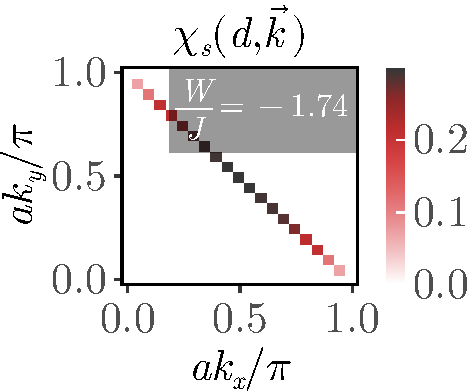
\includegraphics[width=0.49\linewidth]{SF-3.pdf}
    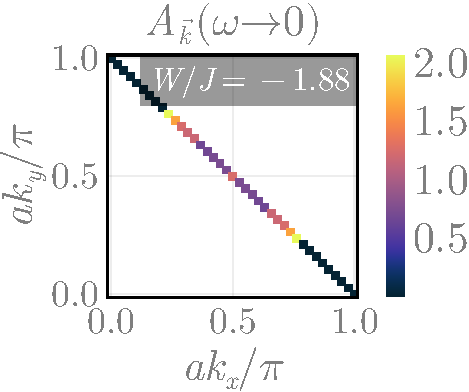
\includegraphics[width=0.49\linewidth]{kspaceDOS-3.pdf}
    \caption{Left: $k-$space resolved spin-spin correlation $\chi_s(d,{\bf k}) = \braket{{\bf S}_d\cdot{\bf S}_{\bf k}}$, in the peudogap phase, confirmed from the fact that only a part of the Fermi surface screens the impurity, the antinodes being the first to decouple from the impurity. This leads, through our tiling relations, to a $k-$space resolved gap on the lattice model, as seen from the DOS (right panel). The region around the antinode of the lattice Fermi surface gets replaced by a Luttinger surface of zeros.}
    \label{spinCorr}
\end{figure}

\paragraph*{Pseudogapping transition from Kondo breakdown.} To obtain various low-energy phases of the impurity model, we perform a scaling analysis of the associated Hamiltonian using the recently developed 
unitary renormalisation group (URG) method \cite{anirbanurg1}. The URG
%method 
proceeds by resolving quantum fluctuations at $T=0$ involving high-energy degrees of freedom in systems of correlated fermions~\cite{santanukagome,1dhubjhep,anirbanmott2,anirbanmott1,siddharthacpi,anirban_kondo,Patra_2023,anirbanurg2}, leading to a low-energy Hamiltonian with renormalised couplings and emergent degrees of freedom. 
%The method has been applied successfully to a variety of problems involving correlated fermions~\cite{santanukagome,1dhubjhep,anirbanmott2,anirbanmott1,siddharthacpi,anirban_kondo,Patra_2023,anirbanurg1,anirbanurg2}; 
We present the results for the present impurity model here, and the details of the calculation are presented in \cite{suppmat}. 
%We find that 
The renormalisation in the %momentum
${\bf k}$-resolved Kondo coupling \(J^{(j)}_{{\bf k}_1, {\bf k}_2}\) at the \(j^\text{th}\) RG step is obtained as
\begin{equation}\begin{aligned}\label{KondoRGequation}
	\Delta J^{(j)}_{{\bf k}_1, {\bf k}_2} = -\sum_{{\bf q} \in \text{PS}} \frac{J^{(j)}_{{\bf k}_2,{\bf q}} J^{(j)}_{{\bf q},{\bf k}_1} + 4J^{(j)}_{{\bf q}, {\bf \bar q}} W_{{\bf \bar q}, {\bf k}_2, {\bf k}_1, {\bf q}}}{\omega - \frac{1}{2}|\varepsilon_j| + J^{(j)}_{{\bf q}}/4 + W_{{\bf q}}/2}~,
\end{aligned}\end{equation}
where \(\varepsilon_j\) is the energy of the shell being decoupled at the \(j^\text{th}\) step, the sum is over all momentum states \({\bf q}\) in the particle sector (PS) of the energy shell \(\varepsilon_j\) (i.e., all states 
%that are 
occupied at \(T=0\) and in the absence of any quantum fluctuations), and  \({\bf \bar q} = {\bf q} + {\boldsymbol \pi}\). The bath interaction coupling $W_{{\bf \bar q}, {\bf k}_2, {\bf k}_1, {\bf q}}$ is found to be marginal under these transformations. While the complexity of the RG equation for $J_{{\bf k}_1, {\bf k}_2}$ (eq.\eqref{KondoRGequation}) is clarified through a detailed numerical evaluation, the structure of the equation is qualitatively similar to its counterpart in a study of the Mott MIT in infinite dimensions~\cite{Mukherjee_2023}. This permits the broad conclusion that for the case of attractive bath interactions $(W<0)$, the frustration of Kondo screening due to charge fluctuations (arising from $W$) lead to the Mott metal-insulator transition.

%As we 
Upon tuning the ratio of the bath and Kondo interactions ($W/J$) from zero to negative values, we observe that the following phases are emergent in the impurity model from the competition between the competing $J$ and $W$ couplings in eq.~\eqref{KondoRGequation}- (i) for $W/J<(W/J)_{\text{PG}}$, a local Fermi liquid phase (where the entirety of the Fermi surface participates in Kondo screening), (ii) for $\frac{W}{J} \in [(\frac{W}{J})_{\text{PG}}, (\frac{W}{J})_c]$, a local pseudogapped phase where disconnected parts of the Fermi surface around the node participate in Kondo screening, and (iii) a local moment phase for $\frac{W}{J} > (\frac{W}{J})_c$, where the impurity remains unscreened at low-energies. These can be visualised from $k-$space resolved spin correlations $\chi_s(d,{\bf k}) = \braket{{\bf S}_d\cdot{\bf S}_{\bf k}}$; see Fig.~\ref{spinCorr} for $\chi_s(d,{\bf k})$ in the PG. The values $(W/J)_{\text{PG}}$ and $(W/J)_c$ are hence defined as the entry into and exit from
%boundaries of 
the pseudogap phase. %Using our 
Upon mapping to the lattice model via tiling, we %consequently 
observe that the $T=0$ Mott transition 
%in $k-$space for 
of the 2D Hubbard-Heisenberg model proceeds from Fermi liquid to Mott insulator through an intervening pseudogap phase
%. obtain an $k$-space pseudogapped phase 
with a partially gapped Fermi surface (i.e., a vanishing electronic density of states around the antinodal regions, Fig.~\ref{spinCorr}, right panel). 
%This constitutes one of the main results of our work, and 
We now lay out the mechanism leading to the formation of the pseudogap. 
%it shows that the breakdown of Kondo screening on the 
%a realistic 2D square lattice very naturally gives rise to a pseudogapped phase with Fermi arc-like behaviour. 
%The local Fermi liquid and local moment phases for the impurity model correspond, respectively, to Fermi liquid and Mott insulating phases on the lattice.

\paragraph*{Unraveling of Kondo screening.} 
% As shown in Fig.~\ref{rgProgression}, the $k-$space anisotropic nature of the Kondo breakdown process 
% %in this model 
% can be visualised in terms of zeros of $J_{{\bf k}_1, {\bf k}_2}$.
% %the Kondo coupling in $k-$space. 
% Consider processes $J_{{\bf k}_N, {\bf k}}$ that involve spin-flip scattering between the node ${\bf k}_N = (\pi/2, \pi/2)$  and a general wavevector ${\bf k}$. 
As shown in Fig.~\ref{rgProgression}, the $k-$space anisotropic nature of the Kondo breakdown process 
can be visualised in terms of zeros of $J_{{\bf k}_N, {\bf k}}$, involving spin-flip scattering between the node ${\bf k}_N = (\pi/2, \pi/2)$  and a general wavevector ${\bf k}$. 
At $W/J=0$, $J_{{\bf k}_N, {\bf k}}$ vanishes if ${\bf k}$ is either any of the antinodes or adjacent nodes. 
%As 
Tuning $W/J$ %is tuned 
towards $(W/J)_{\text{PG}}$ leads to an unraveling of Kondo screening:
%the beginning of the pseudogap, we find that 
$J_{{\bf k}_N, {\bf k}}$ for ${\bf k}$ close to the adjacent nodes turn RG irrelevant first, and a patch of zeros subsequently appears in $J_{{\bf k}_N, {\bf k}}$ around this point (Fig. \ref{rgProgression} (left) panel). %This is the first step towards the decoupling of $J_{{\bf k}_1, {\bf k}_2}$ connecting adjacent quadrants of the Brillouin zone quadrants. 
%that is described in more detail in a later section.
Tuning $W/J$ further extends the patch of zeros
%systematic decoupling of 
in $J_{{\bf k}_1, {\bf k}_2}$ for all ${\bf k}_{1}$ lying between a given node and the nearest antinodes (Fig. \ref{rgProgression} (center) and (right) panels), visualising a systematic decoupling of $J_{{\bf k}_1, {\bf k}_2}$ connecting adjacent quadrants of the Brillouin zone quadrants. 
%via an outwards progression of the patch of zeros 
%from the nodal towards 
%the single zeroes on the nearest antinodal regions . 
Precisely At $W/J=(W/J)_{\text{PG}}$, the antinode joins this connected region of zeros in $J_{{\bf k}_1, {\bf k}_2}$, %and this coincides 
marking (within our numerical precision) to the decoupling of the antinodes from all other points in the neighbourhood of the Fermi surface. This is an interaction-driven Lifshitz transition of the Fermi surface, and marks entry into a pseudogap phase possessing Fermi arcs~\cite{WuFerrero2018}. Importantly, it coincides with an emergent two-channel Kondo impurity model, where each channel corresponds to a pair of Fermi arcs on opposite faces of the conduction bath Fermi surface. 
%At this point, $J(k_N, k)$ is distributed through two disconnected non-zero patches, in the quadrant of $k_N$ and in the opposite quadrant. 
The pseudogap expands by shrinking these disconnected Fermi arcs towards the respective nodes, leading to nodal metals whose disappearance marks the Mott transition. 
%[TODO That the unraveling begins and ends at zeros of the Kondo coupling reveals the role of Fermi surface topology in obtaining the pseudogap~\cite{WuFerrero2018}.]

\begin{figure}[htpb]
    \centering
    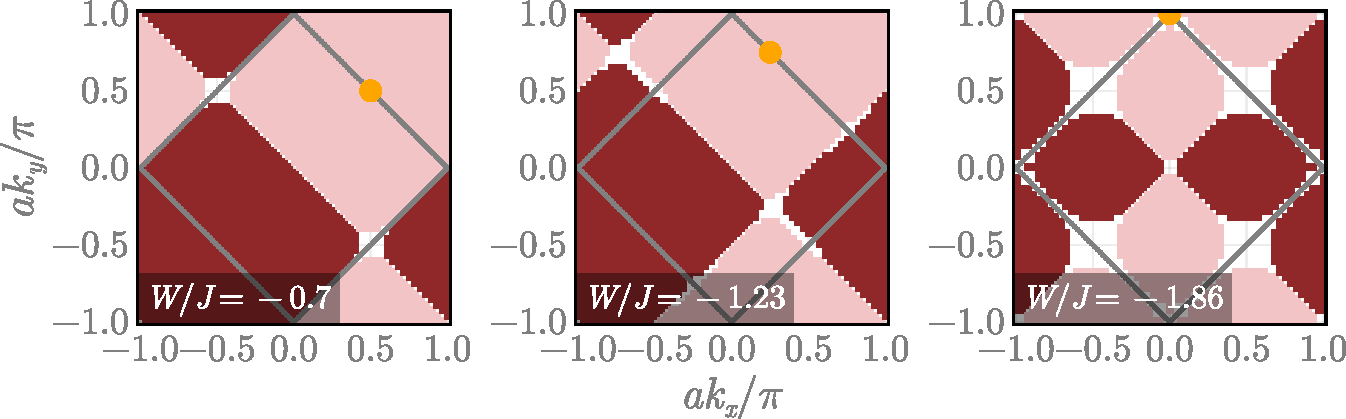
\includegraphics[width=\linewidth]{zerosFlow.pdf}
    \caption{Progression of Kondo couplings into decoupling of adjacent quadrants and the beginning of pseudogap. This is shown by tracking how $J(k_N, k)$ (with $k_N$ pivotted at the top left node and $k$ (depicted as an orange circle) moving along the top right Fermi surface arm) vanishes at different values of $W$ for different values of $k$. The route towards decoupling begins as scattering processes starting from the node and ending at the adjacent node lose spectral weight. This can be seen in the growth of the white zero region at the top left node. As we get closer to the pseudogap, points $k$ in between the node and antinode also decouple from the adjacent node (middle panel). The adjacent quadrant decoupling and onset into the pseudogap is completed by the antinode, which decouples from all points in the neighborhood of the Fermi surface.}
    \label{rgProgression}
\end{figure}

\paragraph*{{\bf k}-resolved dynamical spectral weight transfer.} 
%In order to understand the mechanism driving 
Further insight into the pseudogapping 
%transition 
%in our model, we study 
is obtained from the strong fluctuations observed in charge correlations between the gapless nodal and gapped antinodal regions in this 
%pseudogapped 
regime
%, and find strong fluctuations
(Fig.~\ref{chargeCorr}, left panel). This suggests that the 
%creation of the 
pseudogap in the lattice model
%is brought about by 
emerges from the impurity model from the 
%development 
onset of charge fluctuations in the bath that prohibit correlated spin fluctuations with the impurity spin that
%. Since the latter 
%processes are the ones that give rise 
lead to the 
%central 
Kondo resonance at low-energies in the impurity spectral function. In this way, pseudogap formation 
%is a demonstration of 
results from the transfer of spectral weight from low to high energies. Accordingly, the pseudogap coincides 
%is also seen from 
with the appearance of poles of the lattice model self-energy $\Sigma ({\bf k},\omega=0)$
%in $k-$space  
near the antinodes; these poles approach the nodes 
%as the system is 
upon tuning towards the Mott transition
%through the pseudogap 
(Fig.~\ref{chargeCorr} right panel). The same is observed in the imaginary part of the impurity self-energy of the underlying impurity model~(Fig.\ref{channelDecoupling} (right panel)). 

\begin{figure}
    \centering
    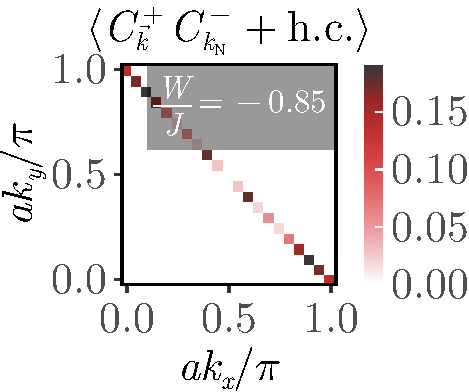
\includegraphics[width=0.49\linewidth]{cfnode-2.pdf}
    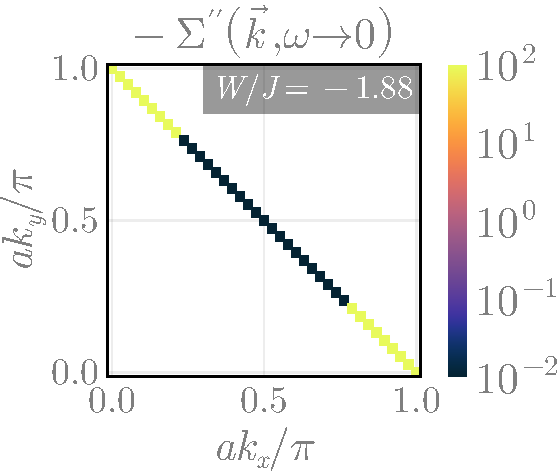
\includegraphics[width=0.49\linewidth]{selfEnergyKspace-3.pdf}
    \caption{Left: Charge isospin correlations $\chi_c({\bf k}_1, {\bf k}_2) = \braket{c^\dagger_{{\bf k}_1\uparrow}c^\dagger_{{\bf k}_1\downarrow}c_{{\bf k}_2\downarrow}c_{{\bf k}_2\uparrow} + \text{h.c.}}$ between the node and other $k-$points, in the pseudogap phase. The enhanced correlations between the node and the antinode suggests that these charge correlations lead to Kondo breakdown. The Kondo breakdown in turn leads to the gapping out of these regions in $k-$space on the lattice model, as seen from the appearance of poles in the imaginary self-enery (right panel).}
    \label{chargeCorr}
\end{figure}

\paragraph*{Non-Fermi liquid nature of the pseudogap.} In the pseudogap regime $|W/J|_{\text{PG}} < |W/J| < |W/J|_{c}$, the nature of the %metal 
gapless Fermi arcs is observed to change dramatically. 
%In this regime, we find that the Kondo couplings $J({\bf k}_1, {\bf k}_2)$ involving momenta from adjacent quadrants of the Brillouin zone are RG-irrelevant, disappearing from the low-energy fixed point Hamiltonian. 
First, we have already argued that the low-energy dynamics of these gapless Fermi arcs are governed by an underlying %simpler 
two-channel Kondo (2CK) impurity model~\cite{Tsvelick_weigmann_mchannel_1985,emery_kivelson}.
%, where the two pairs of opposite Brillouin zones form the two channels. 
Previous works 
%by Coleman and Ioffe
%, as well as one of our own previous works~\cite{Patra2023MCK}, 
show that the impurity self-energy of such a two-channel Kondo model displays marginal Fermi liquid (MFL) behaviour~\cite{Coleman_tsvelik,Schofield1997,Patra2023MCK}: $\Sigma \propto \omega \ln \omega$. The excitations of the 2CK also exhibit a separation of the spin, charge and channel quantum numbers~\cite{affleck1992}, i.e., with gapless excitations carrying only spin quantum number. The non-Fermi liquid nature
%at this also happens in the present model 
is further corroborated by the passage of the impurity quasiparticle residue $Z_\text{imp} = 1/(1 - \frac{\text{d}}{\text{d}\omega}\text{Re}(\Sigma))$ (Fig.~\ref{channelDecoupling} left panel) from finite values in the Fermi liquid phase to vanishingly small values in the pseudogap.
%, where $\Sigma^\prime(\omega)$ is the real part of the impurity self-energy. 
Upon tiling, 
%we can immediately see that 
the resulting MFL metal of the lattice model 
%is arising from such a is not a Fermi liquid; the 
possesses many-particle excitations that involve 
%of the MFL will involve excitations of 
multiple \(k-\)states.

Crucially, we find that passage through the pseudogap phase causes the nature of the non-Fermi liquid to evolve: very near the transition, the excitations of the marginal Fermi liquid %description is found to break down at the transition, and is 
are replaced by 
%those the non-Fermi liquid excitations 
of a Hatsugai-Kohmoto model~\cite{Baskaran1991,Hatsugai1992}. %In order to obtain this, we carry out a 
This insight is obtained from a perturbation-theoretic treatment of the RG fixed point Hamiltonian of the impurity model for $W/J\lesssim (W/J)_{\text{PG}}$,
%in this region of the phase diagram, 
by considering the effects of a small fixed point Kondo scattering probability \(J^*\) in the backdrop of a larger bath interaction parameter \(|W|\). 
%We focus here on 
This yields the HK model~\cite{Baskaran1991,Hatsugai1992} as the singular
%, critical 
part of the effective Hamiltonian arising from forward scattering processes 
%within the complete Hamiltonian 
(details 
%described 
in Appendix~\ref{hkmDerivation}):
\begin{equation}\begin{aligned}\label{HKModel}
	\Delta \tilde H_{{\bf q}_1 = {\bf q}_2} = \sum_{{\bf q},\sigma}\epsilon_{{\bf q}}{n}_{{\bf q},\sigma} + u\sum_{{\bf q}, \sigma}n_{{\bf q} \sigma} n_{{\bf q} \bar\sigma}~,
\end{aligned}\end{equation}
where the number operator \(n_{{\bf q} \sigma} = \phi^\dagger_{{\bf q}, \sigma} \phi_{{\bf q}, \sigma}\) pertains to emergent fermionic modes,
\begin{equation}\begin{aligned}
	\phi_{{\bf q}, \sigma} = \frac{1}{\sqrt 2}\left(c_{{\bf N}_1 + {\bf q},\sigma} - c_{{\bf N}_1 + {\bf Q}_1 - {\bf q}, \sigma}\right)~,
\end{aligned}\end{equation}
that are shifted by an excitation momentum \({\bf q}\) away from the nodal point \({\bf N}_1 = \left(\pi/2, \pi/2\right)\) and its nested partner \({\bf N}_1 + {\bf Q}_1 = \left(-\pi/2, -\pi/2\right)\). The kinetic energy (\(\epsilon_{\bf q}\)) and interaction \(u\) energy scales of the excitations are:
\begin{equation}\begin{aligned}
	\epsilon_{\bf q} = \text{sign}\left(\varepsilon_{{\bf N}_1 + {\bf q}}\right)\frac{\varepsilon_{{\bf N}_1 + {\bf q}}^2}{-W} + \frac{{J^*}^2}{-4W},~u = \frac{{J^*}^2}{4W}~.
\end{aligned}\end{equation}
%Eq.~\ref{HKModel} describes a Hatsugai-Kohmoto (HK) model~\cite{Baskaran1991,Hatsugai1992}, an exactly solvable model of correlated electrons. 
The non-Fermi liquid 
%nature of the gapless 
excitations in the %metallic 
gapless phase of the model 
manifests as
%in the form of 
a divergent one-particle self-energy at the non-interacting Fermi surface~\cite{Phillips2020}:
\begin{equation}\begin{aligned}
	\Sigma_{{\bf q}}(\omega) = -\frac{u^2/4}{\omega - \epsilon_{\bf q}}, ~\Sigma_{\epsilon_{\bf q}=0}(\omega \to 0)  \to \infty~.
\end{aligned}\end{equation}
The zero-frequency pole of this singular metal %continues to 
exists beyond the transition: in the Mott insulating phase, it marks a hard gap in the spectral function for charge excitations. The singular nature of the excitations in this regime can be attributed to the extremely non-local form of the impurity model (arising from the fact that it couples to only the nodal points in $k-$space). This divergent self-energy is consistent with our numerical calculations of the impurity self-energy which showed that the self-energy poles approach the $\omega=0$ point as the system is tuned towards the transition

\begin{figure}
    \centering
    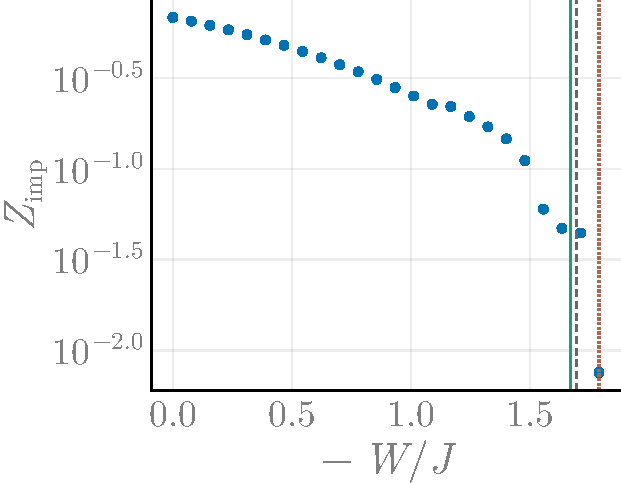
\includegraphics[width=0.49\linewidth]{localQPResidue.pdf}
    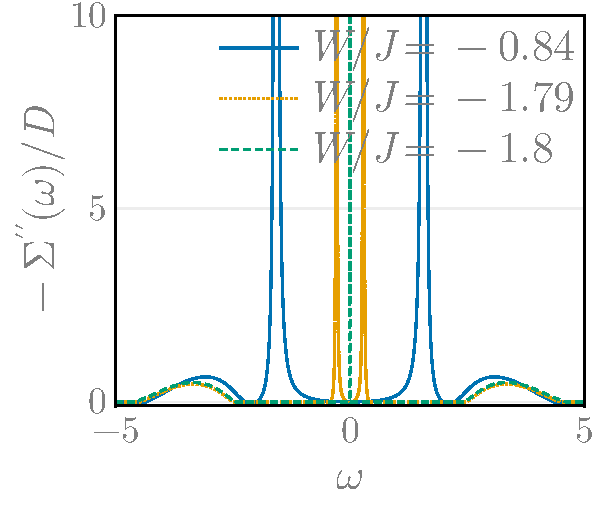
\includegraphics[width=0.49\linewidth]{sigmaImag_49-1000.pdf}
    \caption{Left: Suppression of quasiparticle residue as the system is tuned through various phases. There is an initial abrupt fall at $|W| = |W^*|$, where the system enters the pseudogap and the excitations become non-Fermi liquid. There's a second abrupt fall at the transition due to the presence of a divergent self-energy. Right: Analogous progress of imaginary part of the local self-energy. The poles at the edge of the central Kondo resonance move progressively closer to zero frequency until the Mott pole emerges at zero frequency at the transition.}
    \label{channelDecoupling}
\end{figure}

\paragraph{Morphing of the non-Fermi liquid through the pseudogap}
In order to probe how the metal becomes increasingly correlated as it is tuned through the pseudogap, we compare the quasiparticle residue \(Z_\text{imp}\) and the scattering rate \(\Gamma\) of the quasiparticles, at the beginning and end of the pseudogap. For the regime \(|W| \gtrapprox |W|^*\), the low-energy excitations obey the marginal Fermi liquid theory: \(\Sigma^{\prime} \sim \omega\ln\omega, \Sigma^{\prime\prime}\sim-\omega\). This gives rise to a linear scattering rate \(\Gamma \sim \omega\) (arising from the imaginary part of the self-energy), and a logarithmically vanishing quasiparticle residue~\cite{varma2002singular}
\begin{equation}\begin{aligned}
Z_\text{imp}(\omega) = (1 - \frac{d\Sigma^\prime}{d\omega})^{-1} \sim (c - \ln \omega)^{-1}
\end{aligned}\end{equation}
where \(c\) is a constant. Close to the transition (\(|W| \lesssim |W_c|\)), the low-energy theory is described by a Hatsugai-Kohmoto model, with a diverging self-energy (obtained in eq.~\eqref{HKSelfenergy} above): 
\begin{equation}\begin{aligned}\label{HKSelfenergy}
	\Sigma({\bf k}) = u^2/\left(\omega - \epsilon_{\bf k}\right) = U^2 \left[\mathcal{P}(\frac{1}{\omega - \epsilon_{\bf k}}) - i\pi \delta(\omega - \epsilon_{\bf k})\right]~,
\end{aligned}\end{equation}
where \(\mathcal{P}\left(\cdot\right)\) represents the principal value, and we used the Sokhotski–Plemelj theorem to write down the final expression. For small but non-zero values of \(\omega - \epsilon_{\bf k}\), we get \(Z_\text{imp} \sim \omega^2/U^2 \). The metal near the transition therefore displays a much more rapid vanishing of the quasiparticle residue compared to the logarithmic vanishing for the marginal Fermi liquid. The scattering rate precisely at the surface \(\omega=\epsilon_{\bf k}\), in fact, diverges: \(\Gamma \sim U^2\delta(\omega - \epsilon_{\bf k})\), in contrast to the linearly vanishing scattering rate of the MFL.

The divergence of the self-energy at the transition also mark the onset of the Mott insulator (Fig.~\ref{channelDecoupling}, righ panel). In this way, we have shown that the Fermi liquid must first morph into a marginal Fermi liquid and then into a Hatsugai-Kohmoto non-Fermi liquid before the Mott insulator can emerge. Our calculations also show that beyond the HK terms, the effective Hamiltonian near the transition contains pairing fluctuations: while subdominant at $1/2$-filling, their presence suggests that upon doping away from the Mott insulating state, such a non-Fermi liquid can undergo a superconducting transition. Recent works on the HK model suggest that such a superconductor is likely to be of the non-BCS kind~\cite{Phillips2020}.

Real-space spin-correlations and entanglement within the impurity model (Fig.~\ref{realSpaceCorrelations}) reveal that the spin correlations undergo a crossover within the PG from short-ranged behaviour at the onset to long-ranged behaviour as the Mott transition is approached. [TODO This matches well with similar observations from diagrammatic Monte Carlo simulations of the Hubbard model at finite temperatures, suggesting that the behaviour observed here is generic~\cite{SimkovicFerrero2024}]. the This is further evidence of the breakdown of local Kondo screening and Landau quasiparticles inside the PG. Another implication of these results is that the paradigm governing such a transition is most likely not that of {\it local quantum criticality} - the critical behaviour close to the transition cannot be described by the dynamics of the local sites, and the excitations become truly long-ranged in this regime.

\begin{figure}
    \centering
    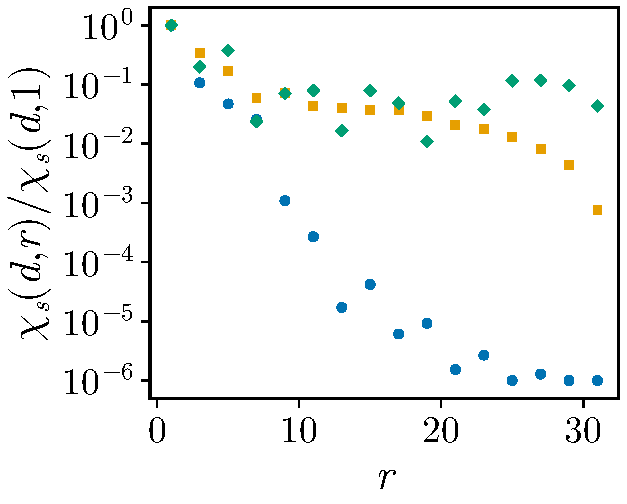
\includegraphics[width=0.49\linewidth]{SF-di_69-2000.pdf}
    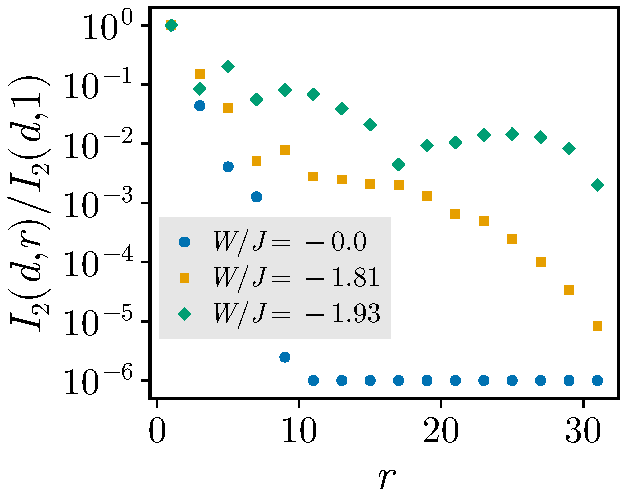
\includegraphics[width=0.49\linewidth]{I2-di_69-2000.pdf}
    \caption{Emergence of long-ranged correlations near the critical point. Left panel: Spin correlations $\chi_s(d,{\bf k}) = \braket{{\bf S}_d^+\cdot{\bf S}_{\bf r}^-}$ between the impurity spin and conduction bath local spins at a distance {\bf r}, as a function of {\bf r}. Right: Mutual information between the same objects, again as a function of the distance. Both decay exponentially fast in the Fermi liquid phase (blue), but show long-ranged behaviour in the non-Fermi liquid phase (green, yellow) and particularly close to the transition (green), indicating that the description of the transition is beyond local quantum criticality.}
    \label{realSpaceCorrelations}
\end{figure}

\paragraph{Luttinger's theorem in the presence of Luttinger surfaces}
One can also ask whether Luttinger's theorem is satisfied in our model in the presence of Luttinger surfaces. It has been shown that particle-hole symmetric systems always satisfy a generalised Luttinger's theorem~\cite{seki2017topological}, where the Fermi volume $V_L$ is represented as the difference in the number of poles and zeros, of the single-particle Greens function, that are enclosed by the Fermi surface~\cite{seki2017topological}. This holds true even in the presence of a divergent self-energy~\cite{Phillips2013}. Since our model is always at half-filling, Luttinger's theorem is always satisfied. 

The way it works out (despite the presence of Luttinger surfaces) is as follows. We need only show that the number of occupied states below the chemical potential remains unchanged across the first Lifshitz transition. Before the transition, the presence of gapless excitations ensures that the Fermi surface is singly-occupied on average. Inside the pseudogap, the gapless $k-$states continue to contribute one pole on average to the Luttinger count, while the gapping out of certain $k-$states leads to a rearrangement of their spectrum: doubly-occupied states on the Luttinger surfaces become more favourable compared to the singly-occupied states (due to the attractive $W$-interaction). Owing to particle-hole symmetry, these states are degenerate with the zero occupancy states, so that on average, a single state is again occupied. This ensures that the number of occupied states (and hence the number of occupied poles) remains unchanged across the transition. The same argument works for the Mott insulator, where the entire Fermi surface gets replaced by a Luttinger surface.

\paragraph*{Acknowledgements}
AM thanks IISER Kolkata for funding through a JRF and SRF. S Lal thanks the SERB, Govt. of India for funding through MATRICS Grant MTR/2021/000141 and Core Research Grant CRG/2021/000852.

\appendix

\section{Appendixes}

\bibliography{tilingProject}% Produces the bibliography via BibTeX.

\end{document}